\thispagestyle{lichsutoanhocnone}
\pagestyle{lichsutoanhoc}
\graphicspath{{../lichsutoanhoc/pic/}}
\everymath{\color{lichsutoanhoc}}
\blfootnote{$^1$\color{lichsutoanhoc}Cộng tác viên Viện Toán học.}
\begingroup
\AddToShipoutPicture*{\put(0,616){\includegraphics[width=19.3cm]{../bannerlichsu}}}
\AddToShipoutPicture*{\put(48,437){\includegraphics[scale=1]{../tieude.pdf}}}
\centering
\endgroup

\vspace*{272pt}

\begin{multicols}{2}
	\textbf{\color{lichsutoanhoc}Dẫn nhập}
	\vskip 0.05cm
	Nếu Thales (khoảng $625-547$ trước Công nguyên--TCN) và Pythagoras (khoảng $584-495$ TCN) là những người đặt nền móng cho sự phát triển một nghìn năm toán học Hy Lạp thì Euclid (khoảng $330-275$ TCN) và  Archimedes (khoảng $287-212$ TCN) là những đỉnh cao của Toán học Hy Lạp nói riêng và Toán học nói chung. Trong bộ sách đồ sộ \textit{Elements (Cơ sở)}  gồm $13$ quyển, được dùng trong $2000$ năm, được tái bản nhiều lần với sửa chữa rất ít và sự phổ biến chỉ kém Kinh thánh, Euclid đã tiếp thu, hoàn thiện, hệ thống và phát triển toàn bộ kiến thức toán học thế giới đã đạt được trước đó, trong đó có thành tựu toán học Hy Lạp trong $300$ năm từ thế kỷ V đến thế kỷ III trước Công nguyên. 
	\vskip 0.05cm
	Bài viết này giới thiệu những bài toán và kiến thức cơ bản đạt được bởi các nhà toán học Hy Lạp sau Pythagoras và trước Euclid. Ở một số chỗ, bài viết cũng liên hệ các thành tựu toán học thời kỳ này với Cơ sở của Euclid và toán học các thời kỳ sau.    
	\vskip 0.05cm
	\textbf{\color{lichsutoanhoc}Ba bài toán kinh điển: cầu phương hình tròn, chia ba một góc và gấp đôi thể tích lập phương}
	\vskip 0.05cm
	Ba bài toán này đã thu hút các nhà toán học suốt $2000$ năm. Ở đây chúng ta thấy một toán học khác hoàn toàn với toán học Babilon và toán học Ai Cập. Đây không còn là ứng dụng thực tế của số học vào các vấn đề của đời sống, mà là sự phát triển toán học dựa trên nền tảng vững chắc  của suy luận, chứng tỏ sự khác biệt rõ ràng giữa các bài toán thực tế với phát triển tư duy và phát triển nội tại của toán học.
	\vskip 0.05cm
	\textbf{\color{lichsutoanhoc}Bài toán cầu phương hình tròn}
	\vskip 0.05cm
	Theo Plutarch ($46-119$ CN), trong thời gian ở trong tù, Anaxagoras (khoảng $500-428$ TCN) đã tìm cách giải bài toán cầu phương hình tròn, tức là bài toán dựng hình bằng thước và compa biến hình tròn thành hình vuông có cùng diện tích. 
	\vskip 0.05cm
	Nếu $r$ là bán kính hình tròn cho trước thì diện tích của nó bằng $\pi r^2$. Diện tích hình vuông cạnh $a$  là $a^2$. Suy ra  $a^2 = \pi r^2$ hay  $a=\sqrt{\pi}r$. Bài toán trở thành: Cho trước hai điểm $A,B$. Hãy dựng điểm $C$  trên đường thẳng  $AB$  sao cho $AC = \sqrt{r}AB$  hay $a= \sqrt{\pi}r$.
	\vskip 0.05cm 
	\textbf{\color{lichsutoanhoc}Bài toán gấp đôi thể tích hình lập phương}
	\vskip 0.05cm
	Anaxagoras mất vào năm $428$ TCN, đúng một năm trước khi Plato sinh ra và một năm sau Pericles mất. Tương truyền rằng Pericles chết vì bệnh dịch hạch, một bệnh dịch đã làm chết một phần tư dân số Athens, và thảm họa này đã là nguồn gốc cho bài toán toán học nổi tiếng thứ hai. Một phái đoàn Athens được cử đến nhà tiên tri của thần Apollo tại Delos để hỏi làm cách nào để ngăn chặn bệnh, và nhà tiên tri đã trả lời rằng bàn thờ hình khối lập phương cho thần Apollo phải được tăng gấp đôi về thể tích. Người Athens đã tăng gấp đôi kích thước của bàn thờ, nhưng bệnh dịch vẫn hoành hoành. Tất nhiên, bàn thờ đã được tăng gấp tám lần về thể tích, thay vì gấp hai lần như yêu cầu. Đây chính là bài toán: \textit{Dựng bằng thước và compa một cạnh của khối lập phương có thể tích gấp đôi khối đã cho.}
	\vskip 0.05cm
	Giả sử  $a$ là cạnh của lập phương đã cho,  $b$ là cạnh của lập phương cần tìm. Theo yêu cầu, ta có $b^3 = 2a^3$, tức là $b = \sqrt[3]{2}a$.  Bài toán trở thành: Cho hai điểm $A,B$. Tìm điểm  $C$ trên đường thẳng $AB$  sao cho $AC = \sqrt[3]{2}AB$  hay $b = \sqrt[3]{2}a$.
	\vskip 0.05cm 
	\textbf{\color{lichsutoanhoc}Bài toán chia ba một góc}
	\vskip 0.05cm
	Trong thời gian đó, lan truyền ở Athens một bài toán thứ ba cũng nổi tiếng không kém: Hãy dựng một góc bằng một phần ba góc đã cho nhờ thước kẻ và compa. Bài toán được phát biểu như sau: Cho hai điểm $A,B$ tùy ý trên đường tròn tâm $O$.  Tìm điểm $C$ trên cung $AB$ sao cho $\angle AOC = \dfrac{1}{3} \angle AOB$.
	\vskip 0.05cm  
	Ba bài toán: cầu phương hình tròn, gấp đôi thể tích hình lập phương và bài toán chia ba một góc là ba bài toán nổi tiếng (ba bài toán kinh điển) của thời cổ đại. Để chứng minh cả ba bài toán này đều không giải được nếu chỉ dùng thước và compa, phải dùng đến lý thuyết trường. Điều này đã được các nhà toán học thế kỷ XIX (Lindemann,  Gauss, Wanzel, \ldots) giải quyết trọn vẹn.  
	\vskip 0.05cm
	\textbf{\color{lichsutoanhoc}Hippocrates: Bài toán cầu phương hình tròn  và Diện tích hình trăng khuyết}
	\begin{figure}[H]
		\vspace*{-5pt}
		\centering
		\captionsetup{labelformat= empty, justification=centering}
		\includegraphics[width= 0.65\linewidth]{1}
		\caption{\small\textit{\color{lichsutoanhoc}Hippocrates ($460-380$ TCN).}}
		\vspace*{-10pt}
	\end{figure}
	Nhà toán học lỗi lạc nhất Hy Lạp vào nửa sau thế kỷ V là Hippocrates xứ Chios. ông sống vào khoảng $460-380$ TCN,  hơi trẻ hơn Anaxagoras. Cần phân biệt ông  với bác sĩ nổi tiếng cùng tên và cùng thời Hippocrates xứ Cos (khoảng $460-370$ TCN). Giống như Thales, Hippocrates đã khởi nghiệp như một thương gia và trở thành nhà nghiên cứu toán học vào cuối đời. Aristotle cho rằng Hippocrates kém sắc sảo hơn Thales và do đó ông ta đã bị lừa hoặc bị cướp khi đi buôn. Hippocrates đã đến Athens để theo kiện. Phải ở lại Athens trong nhiều năm (vào khoảng những năm $430$ TCN), ông đã tham dự các bài giảng của một số triết gia. Có lý do để tin rằng những người Pythagoras (những người theo trường phái Pythagoras) đã định cư ở Athens vào thời điểm đó, vì vậy ông có thể đã học họ mặc dù ông không có thầy chính thức là người Pythagoras. Cuối cùng, Hippocrates đã đạt được trình độ cao trong hình học đến mức ông trở thành một trong những người đầu tiên kiếm được tiền bằng dạy toán. Những người Pythagoras đã dạy ông những gì họ biết về số học và hình học, sau đó ông đã phản bội lòng tin của họ bằng cách bán những bí mật toán học của người Pythagoras cho bất kỳ ai mua (một cách giải thích nhẹ nhàng hơn là người Pythagoras, cảm thông với sự bất hạnh của Hippocrates, đã cho phép ông kiếm tiền bằng cách dạy các kiến thức hình học của họ).
	\vskip 0.05cm
	Hippocrates coi thất bại trong kinh doanh là vận may của ông, vì ông đã có cơ hội tập trung nghiên cứu hình học, ở đó ông đã đạt được thành công đáng kể. 
	\vskip 0.05cm
	Vào giữa thế kỷ thứ V, rất nhiều định lý hình học đã được thiết lập dẫn tới sự cần thiết phải đưa tất cả kiến thức này vào một trật tự logic tốt. Proclus viết rằng Hippocrates đã viết cuốn  \textit{Cơ sở của hình học}, trước hơn một thế kỷ cuốn \textit{Cơ sở}  của Euclid. Tuy nhiên, cuốn sách của Hippocrates đã bị thất lạc, mặc dù nó đã được Aristotle ($384-322$ TCN) nói đến. Cuốn sách của Hippocrates có thể đã bắt đầu một truyền thống viết sách đáng chú ý, nhưng nó có những thiếu sót của một tác phẩm tiên phong, và do đó đã bị lỗi thời trước \textit{Cơ sở} của Euclid.
	\vskip 0.05cm
	Hippocrates đã trình bày hình học như một chuỗi các mệnh đề, một hình thức trình bày giống như cách trình bày hiện đại, trong đó các mệnh đề cần chứng minh có thể được suy ra trên cơ sở của những mệnh đề trước đó. Trong số những đổi mới khác, ông đã sử dụng các chữ cái để ký hiệu các điểm và đường trong các hình hình học.
	\vskip 0.05cm
	Khi Hippocrates đến Athens, ba bài toán--cầu phương hình tròn, nhân đôi thể tích của khối lập phương và chia ba một góc--đã thu hút sự chú ý của các nhà hình học. Những bài toán này là các bài toán kinh điển trong lịch sử toán học, là  nguồn kích thích và say mê giống nhau cho những người nghiệp dư và học giả qua các thời đại, cho đến tận thế kỷ XIX và thậm chí cho tới thế kỷ XX, do không hiểu những bài toán này không thể giải được bằng thước và compa, nhiều nhà toán học nghiệp dư vẫn say sưa ``cầu phương hình tròn."
	\vskip 0.05cm
	Trong thực tế, không có tác phẩm toán học nào từ thế kỷ V TCN còn tồn tại, nhưng còn một chứng cớ là Simplicius (khoảng năm $520$ CN) tuyên bố đã sao chép theo nghĩa đen cuốn  \textit{Lịch sử Toán học} (đã mất) của Eudemus. Từ tuyên bố ngắn gọn này, chúng ta biết Hippocrates đã giải bài toán cầu phương hình trăng khuyết (hình giới hạn bởi hai cung tròn có bán kính không bằng nhau). Vấn đề cầu phương hình trăng khuyết chắc chắn đã nảy sinh từ bài toán cầu phương hình tròn và dựa trên khẳng định (của Hippocrates): \textit{Tỷ lệ diện tích các hình tròn có cùng tỷ lệ với các hình vuông nội tiếp các hình tròn ấy.}
	\vskip 0.05cm
	Ở đây Hippocrates đã sử dụng ngôn ngữ và khái niệm về tỷ lệ đóng một vai trò rất lớn trong tư tưởng của người Pythagoras. Trên thực tế, một số người cho rằng Hippocrates đã trở thành người theo trường phái Pythagoras. Trường Pythagoras ở Crotone đã bị đóng cửa, phái Pythagoras bị đàn áp (có thể vì tính bí mật, cũng có thể vì xu hướng chính trị bảo thủ của nó), nhưng sự phân tán của những người Pythagoras trên khắp thế giới tiếng Hy Lạp lại mở rộng ảnh hưởng của trường phái Pythagoras. Không nghi ngờ gì nữa, điều này đã ảnh hưởng, trực tiếp hoặc gián tiếp, tới Hippocrates.
	\vskip 0.05cm
	Trong mảnh sách còn lại của Eudemus có hai định lý sau (được coi là của Hippocrates). 
	\vskip 0.05cm
	\textbf{\color{lichsutoanhoc}Định lý} $\pmb{1.}$ Giả sử $AB$  là đường kính hình tròn tâm  $D$, $AC$  và $BC$  là hai cạnh của  hình vuông nội tiếp trong hình tròn ấy. Dựng nửa đường tròn $AEC$  đường kính  $AC$. Khi ấy diện tích hình trăng khuyết $AECFA$  bằng diện tích tam giác  $ADC$ (Hình $1a$).
	\begin{figure}[H]
%		\vspace*{-5pt}
		\centering
		\captionsetup{labelformat= empty, justification=centering}
		\begin{tikzpicture}
			\draw [shift={(2.5,0.)},lichsutoanhoc]  plot[domain=0.:3.141592653589793,variable=\t]({1.*2.5*cos(\t r)+0.*2.5*sin(\t r)},{0.*2.5*cos(\t r)+1.*2.5*sin(\t r)});
			\draw [lichsutoanhoc] (0.,0.)-- (5.,0.);
			\draw [shift={(1.25,1.25)},lichsutoanhoc]  plot[domain=0.7853981633974483:3.9269908169872414,variable=\t]({1.*1.7677669529663689*cos(\t r)+0.*1.7677669529663689*sin(\t r)},{0.*1.7677669529663689*cos(\t r)+1.*1.7677669529663689*sin(\t r)});
			\draw [lichsutoanhoc] (2.5,2.5)-- (0.,0.);
			\draw [lichsutoanhoc] (2.5,2.5)-- (5.,0.);
			\draw [lichsutoanhoc] (2.5,2.5)-- (2.5,0.);
				\draw [fill=white] (0.,0.) circle (1.5pt);
				\draw[color=lichsutoanhoc] (-0.18,-0.19) node {$A$};
				\draw [fill=white] (5.,0.) circle (1.5pt);
				\draw[color=lichsutoanhoc] (5.16,-0.27) node {$B$};
				\draw[color=lichsutoanhoc] (1.12,2.47) node {$F$};
				\draw [fill=white] (2.5,0.) circle (1.5pt);
				\draw[color=lichsutoanhoc] (2.46,-0.23) node {$D$};
				\draw [fill=white] (2.5,2.5) circle (1.5pt);
				\draw[color=lichsutoanhoc] (2.64,2.83) node {$C$};
				\draw[color=lichsutoanhoc] (-0.12,2.89) node {$E$};
		\end{tikzpicture}
		\caption{\small\textit{\color{lichsutoanhoc}Hình $1a$.}}
		\vspace*{-10pt}
	\end{figure}
	\setlength{\abovedisplayskip}{6pt}
	\setlength{\belowdisplayskip}{6pt}
	\textit{Chứng minh}. Nối $C$ với $D$. Ký hiệu, thí dụ, ${S_{\bigcirc ACB}}$  là diện tích nửa hình tròn $ACB$ đường kính $AB$. Vì $AB^2 = 2AC^2$  (Hình $1a$)  nên 
	\begin{align*}
		\frac{{{S_{\bigcirc ACB}}}}{{{S_{\bigcirc AEC}}}} = \frac{{\pi {{\left( {\frac{{AB}}{2}} \right)}^2}}}{{\pi {{\left( {\frac{{AC}}{2}} \right)}^2}}} = \frac{{A{B^2}}}{{A{C^2}}} = 2
	\end{align*}
	hay ${S_{\bigcirc ACB}} = 2{S_{\bigcirc AEC}}.$
	\vskip 0.05cm
	Nhưng  ${S_{\bigcirc ACB}} = {S_{\bigcirc ADC}} + {S_{\bigcirc BDC}} = 2{S_{\bigcirc ADC}}$ nên ${S_{\bigcirc AEC}} = {S_{\bigcirc ADC}}$.   Suy ra 
	\begin{align*}
		{S_{AECFA}} + {S_{AFCA}} = {S_{AECA}} = {S_{AFCA}} + {S_{\Delta ADC}}.
	\end{align*}
	Vậy diện tích hình trăng khuyết $AECFA$  bằng diện tích tam giác $ADC$,  hay trăng khuyết $AECFA$  đã được ``cầu phương".
	\vskip 0.05cm
	Một phiên bản khác của Định lý $1$ là
	\vskip 0.05cm
	\textbf{\color{lichsutoanhoc}Định lý} $\pmb{1'.}$ Dựng trên các cạnh của tam giác $ABC$ vuông ở $C$   các nửa đường tròn  đường kính $AB, AC, BC$. Khi ấy tổng diện tích hình trăng khuyết $L_1$  và $L_2$ bằng diện tích tam giác  $ABC$ (Hình $1b$).   
	\begin{figure}[H]
		\vspace*{-5pt}
		\centering
		\captionsetup{labelformat= empty, justification=centering}
		\begin{tikzpicture}[scale=0.8]
			\draw [shift={(2.5,0.)},lichsutoanhoc]  plot[domain=0.:3.141592653589793,variable=\t]({1.*2.5*cos(\t r)+0.*2.5*sin(\t r)},{0.*2.5*cos(\t r)+1.*2.5*sin(\t r)});
			\draw [lichsutoanhoc] (0.,0.)-- (5.,0.);
			\draw [lichsutoanhoc] (3.390811455834727,2.33590559529995)-- (0.,0.);
			\draw [lichsutoanhoc] (3.390811455834727,2.33590559529995)-- (5.,0.);
			\draw [shift={(1.6954057279173635,1.167952797649975)},lichsutoanhoc]  plot[domain=0.6032325047411791:3.744825158330972,variable=\t]({1.*2.058765241544895*cos(\t r)+0.*2.058765241544895*sin(\t r)},{0.*2.058765241544895*cos(\t r)+1.*2.058765241544895*sin(\t r)});
			\draw [shift={(4.195405727917364,1.167952797649975)},lichsutoanhoc]  plot[domain=-0.9675638220537177:2.1740288315360754,variable=\t]({1.*1.418268550101352*cos(\t r)+0.*1.418268550101352*sin(\t r)},{0.*1.418268550101352*cos(\t r)+1.*1.418268550101352*sin(\t r)});
			\draw [shift={(2.5,0.)},lichsutoanhoc]  plot[domain=-3.141592653589793:0.,variable=\t]({1.*2.5*cos(\t r)+0.*2.5*sin(\t r)},{0.*2.5*cos(\t r)+1.*2.5*sin(\t r)});
				\draw [fill=white] (0.,0.) circle (1.5pt);
				\draw[color=lichsutoanhoc] (-0.26,-0.13) node {$A$};
				\draw [fill=white] (5.,0.) circle (1.5pt);
				\draw[color=lichsutoanhoc] (5.16,-0.27) node {$B$};
				\draw[color=lichsutoanhoc] (2.56,-0.15) node {$c$};
				\draw [fill=white] (3.390811455834727,2.33590559529995) circle (1.5pt);
				\draw[color=lichsutoanhoc] (3.54,2.71) node {$C$};
				\draw[color=lichsutoanhoc] (2.24,1.19) node {$b$};
				\draw[color=lichsutoanhoc] (3.78,1.45) node {$a$};
				\draw [fill=white] (1.6954057279173635,1.167952797649975) circle (1.5pt);
				\draw[color=lichsutoanhoc] (1.53,1.62) node {$S_1$};
				\draw [fill=white] (4.195405727917364,1.167952797649975) circle (1.5pt);
				\draw[color=lichsutoanhoc] (4.21,1.68) node {$S_2$};
				\draw[color=lichsutoanhoc] (0.75,2.86) node {$L_1$};
				\draw[color=lichsutoanhoc] (5.17,2.) node {$L_2$};
		\end{tikzpicture}
		\caption{\small\textit{\color{lichsutoanhoc}Hình $1b$.}}
%		\vspace*{-5pt}
	\end{figure}
	\textit{Chứng minh}. Ta có   
	\begin{align*}
			{S_{\bigcirc AC}} + {S_{\bigcirc BC}} &= \pi {\left( {\frac{{AC}}{2}} \right)^2} + \pi {\left( {\frac{{BC}}{2}} \right)^2}\\
			&= \frac{\pi }{4}\left( {A{C^2} + B{C^2}} \right) \\
			&= \frac{\pi }{4}A{B^2} = {S_{\bigcirc ABC}}.
	\end{align*}
	Hay (Hình $1b$)
	\begin{align*}
		{S_{{L_1}}} + {S_{{S_1}}} + {S_{{L_2}}} + {S_{{S_2}}} = {S_{\Delta ABC}} + {S_{{S_1}}} + {S_{{S_2}}}.
	\end{align*}
	Suy ra
	\begin{align*}
		{S_{{L_1}}} + {S_{{L_2}}} = {S_{\Delta ABC}}.
	\end{align*}
	\textbf{\color{lichsutoanhoc}Định lý} $\pmb{2}.$ Diện tích nửa lục giác đều $CEFD$ bằng tổng diện tích nửa hình tròn $ALB$  và ba hình trăng khuyết $CGEMC$,  $EHFNE$, $FKDOF$ (Hình $2$).
	\begin{figure}[H]
		\vspace*{-10pt}
		\centering
		\captionsetup{labelformat= empty, justification=centering}
		\begin{tikzpicture}[scale=0.7]
			\draw [lichsutoanhoc] (-5.,0.)-- (-3.,0.);
			\draw [shift={(-4.,0.)},lichsutoanhoc]  plot[domain=0.:3.141592653589793,variable=\t]({1.*1.*cos(\t r)+0.*1.*sin(\t r)},{0.*1.*cos(\t r)+1.*1.*sin(\t r)});
			
			\draw [fill=white] (-5.,0.) circle (1.5pt);
			\draw[color=lichsutoanhoc] (-4.86,0.37) node {$A$};
			\draw [fill=white] (-3.,0.) circle (1.5pt);
			\draw[color=lichsutoanhoc] (-2.86,0.37) node {$B$};
			
			\draw[color=lichsutoanhoc] (-3.82,1.29) node {$L$};
		\end{tikzpicture}
		\caption{\small\textit{\color{lichsutoanhoc}Hình $2a$.}}
		\vspace*{-10pt}
	\end{figure}
	\begin{figure}[H]
		\vspace*{-10pt}
		\centering
		\captionsetup{labelformat= empty, justification=centering}
		\begin{tikzpicture}[scale=0.7]
			\draw [lichsutoanhoc] (-1.,0.)-- (5.,0.);
			\draw [shift={(2.,0.)},lichsutoanhoc]  plot[domain=0.:3.141592653589793,variable=\t]({1.*3.*cos(\t r)+0.*3.*sin(\t r)},{0.*3.*cos(\t r)+1.*3.*sin(\t r)});
			\draw [shift={(-0.25,1.299038105676658)},lichsutoanhoc]  plot[domain=1.0471975511965979:4.188790204786391,variable=\t]({1.*1.5*cos(\t r)+0.*1.5*sin(\t r)},{0.*1.5*cos(\t r)+1.*1.5*sin(\t r)});
			\draw [shift={(2.,2.598076211353316)},lichsutoanhoc]  plot[domain=0.:3.141592653589793,variable=\t]({1.*1.5*cos(\t r)+0.*1.5*sin(\t r)},{0.*1.5*cos(\t r)+1.*1.5*sin(\t r)});
			\draw [shift={(4.25,1.299038105676658)},lichsutoanhoc]  plot[domain=-1.0471975511965983:2.0943951023931953,variable=\t]({1.*1.5*cos(\t r)+0.*1.5*sin(\t r)},{0.*1.5*cos(\t r)+1.*1.5*sin(\t r)});
			\draw [lichsutoanhoc] (-1.,0.)-- (0.5,2.598076211353316);
			\draw [lichsutoanhoc] (0.5,2.598076211353316)-- (3.5,2.598076211353316);
			\draw [lichsutoanhoc] (3.5,2.598076211353316)-- (5.,0.);
		
				\draw [fill=white] (-1.,0.) circle (1.5pt);
				\draw[color=lichsutoanhoc] (-1.08,-0.33) node {$C$};
				\draw [fill=white] (5.,0.) circle (1.5pt);
				\draw[color=lichsutoanhoc] (5.2,-0.29) node {$D$};
				\draw [fill=white] (0.5,2.598076211353316) circle (1.5pt);
				\draw[color=lichsutoanhoc] (0.6,2.31) node {$E$};
				\draw [fill=white] (3.5,2.598076211353316) circle (1.5pt);
				\draw[color=lichsutoanhoc] (3.32,2.33) node {$F$};
				\draw[color=lichsutoanhoc] (-1.72,2.39) node {$G$};
				\draw[color=lichsutoanhoc] (1.98,4.53) node {$H$};
				\draw[color=lichsutoanhoc] (5.72,2.35) node {$K$};
				\draw[color=lichsutoanhoc] (-0.84,1.87) node {$M$};
				\draw[color=lichsutoanhoc] (2.,3.43) node {$N$};
				\draw[color=lichsutoanhoc] (4.86,1.65) node {$O$};
		\end{tikzpicture}
		\caption{\small\textit{\color{lichsutoanhoc}Hình $2b$.}}
		\vspace*{-5pt}
	\end{figure}
	\textit{Chứng minh}. Dựng nửa hình tròn đường kính $AB = \dfrac{1}{2}CD$ (Hình $2a$). Dựng các nửa hình tròn đường kính $CE, EF, FD$ là ba cạnh liên tiếp của lục giác đều nội tiếp đường tròn đường kính  $CD$ (Hình $2b$). Vì 
	\begin{align*}
		C{D^2} = 4A{B^2} = A{B^2} + C{E^2} + E{F^2} + F{D^2}
	\end{align*}
	và tỷ lệ diện tích các hình tròn bằng tỷ lệ diện tích các hình vuông dựng trên đường kính của chúng nên 
	\begin{align*}
		&{S_{\bigcirc CEFD}} \\
		= &{S_{\bigcirc ALB}} + {S_{\bigcirc CGE}} + {S_{\bigcirc EHF}} + {S_{\bigcirc FKD}}.
	\end{align*}
	Trừ hai vế cho tổng diện tích ba hình viên phân $CMEC, ENFE, FODF$  ta được  
	\begin{align*}
		&{S_{CEFD}} \\
		= &{S_{\bigcirc ALB}} + {S_{CGEMC}} + {S_{EHFNE}} + {S_{FKDOF}}.
	\end{align*}
	Eudemus tin rằng Hippocrates đã chứng minh hai định lý trên, nhưng một chứng minh nghiêm túc vào thời điểm đó (khoảng năm $430$ trước Công nguyên) dường như khó có thể xảy ra. Chứng minh trong Quyển $12$ Chương $2$ \textit{Cơ sở} của Euclid dường như là của Eudoxus, một nhà toán học sống nửa thời gian giữa Hippocrates và Euclid. Tuy nhiên, hai cuốn sách đầu của Euclid dường như bắt nguồn từ Pythagoras, vì vậy sẽ có vẻ hợp lý khi giả định rằng công thức, ít nhất, phần lớn cuốn sách III và IV của \textit{Cơ sở}  là từ tác phẩm của Hippocrates. Hơn nữa, nếu Hippocrates đã đưa ra một chứng minh định lý về diện tích của các hình giới hạn bởi các hình tròn, thì Hippocrates chính là người phát minh ra phương pháp chứng minh gián tiếp trong toán học. 
	\vskip 0.05cm
	Từ các định lý về diện tích hình trăng khuyết, Hippocrates được coi là người đầu tiên trong lịch sử toán học tìm ra cách tính diện tích các hình cong (khác hình tròn). 
	\vskip 0.05cm
	Có cơ sở tương đối vững chắc về mặt lịch sử  khi nói rằng cầu phương hình tròn đã được phát triển bởi Hippocrates. Các học giả ngoài Simplicius cũng đề cập đến tác phẩm của Hippocrates. Simplicius sống ở thế kỷ VI, nhưng ông không chỉ trích dẫn Eudemus (khoảng năm $320$ TCN) mà còn dựa vào Alexander xứ Aphrodisias (khoảng năm $200$ CN), một trong những nhà bình luận chính về Aristotle. 
	Các kết quả trên dường như đã khuyến khích Hippocrates, cũng như những người cùng thời và những người kế nhiệm ông hi vọng rằng cuối cùng hình tròn sẽ được cầu phương.
	\vskip 0.05cm
	Các kết quả của Hippocrates về cầu phương hình trăng khuyết có thể coi là những nỗ lực đáng kể của toán học vào thời điểm đó. Nó cho thấy rằng các nhà toán học Athens rất thành thạo trong việc xử lý các phép biến đổi diện tích và tỷ lệ.
	\vskip 0.05cm 
	Có ba quan điểm về những gì Hippocrates đã suy luận từ cầu phương hình trăng khuyết. Một số đã buộc tội ông vì tin rằng ông có thể cầu phương tất cả các hình trăng, trong đó có hình tròn; Những người khác nghĩ rằng ông biết những hạn chế công việc của mình, biết rằng nó được chứng minh chỉ với một số loại hình trăng. Một học giả lại viết rằng Hippocrates biết ông đã không cầu phương hình tròn nhưng cố đánh lừa đồng hương là mình đã thành công. 
	\vskip 0.05cm
	Hippocrates còn là người đầu tiên sử dụng ký hiệu chữ cái trong các hình hình học. Thật thú vị khi lưu ý rằng trong khi Hippocrates có đóng góp trong hai bài toán nổi tiếng, ông dường như đã không có tiến bộ trong bài toán chia ba một góc, một vấn đề được nghiên cứu phần nào sau đó bởi Hippias của Elis.
	\vskip 0.05cm
	\textbf{\color{lichsutoanhoc}Hippias xứ Elis}
	\vskip 0.05cm
	Vào cuối thế kỷ thứ năm TCN, một nhóm giáo viên chuyên nghiệp hoàn toàn không giống như người Pythagoras nổi lên mạnh mẽ ở Athens. Trong số này có Hippias, một người gốc Elis, đã sống tại Athens vào nửa sau của thế kỷ thứ năm TCN.  ông là một trong những nhà toán học đầu tiên mà chúng ta có thông tin trực tiếp, vì chúng ta đọc được nhiều điều về ông từ \textit{Đối thoại} của Plato. ông được cho là đã viết nhiều, từ toán học để diễn xướng, nhưng không có tác phẩm nào của ông còn tồn tại.  
	\vskip 0.05cm
	Hippias (khoảng $500-401$ TCN)  sống cùng thời với Socrates (khoảng $477-399$ TCN). Socrates được cho là đã mô tả Hippias đẹp trai, học giỏi nhưng khoe khoang và nông nổi. Trong \textit{Đối thoại} của Plato và \textit{Những kỷ vật} của Xenophon có những nhận xét không mấy hay ho về Hippias như một người tự coi mình là một chuyên gia trong mọi thứ từ lịch sử và văn học đến thủ công mỹ nghệ và khoa học. 
	\vskip 0.05cm
	Proclus và các nhà toán học khác đã gán tên trisectrix hoặc quadratrix cho Hippias, các đường cong khác đường tròn và đường thẳng. Điều này được mô tả như sau: Trong hình vuông $ABCD$ (Hình $3$), cho cạnh $AB$ di chuyển đều từ vị trí hiện tại của nó cho đến khi nó trùng với $DC$ và để chuyển động này diễn ra chính xác cùng thời gian $DA$ quay theo chiều kim đồng hồ từ vị trí hiện tại của nó cho đến khi nó trùng với $DC$.
	\begin{figure}[H]
		\vspace*{-10pt}
		\centering
		\captionsetup{labelformat= empty, justification=centering}
		\begin{tikzpicture}[color=lichsutoanhoc,scale=0.8]
			\draw  (0,5)-- (5,5);
			\draw  (5,5)-- (5,0);
			\draw  (5,0)-- (0,0);
			\draw  (0,0)-- (0,5);
			\draw [dashed] (0,1)-- (5,1);
			\draw [dashed] (0,2)-- (5,2);
			\draw  (0,3)-- (5,3);
			\draw [shift={(0,0)}]  plot[domain=0:1.5707963267948966,variable=\t]({1*5*cos(\t r)+0*5*sin(\t r)},{0*5*cos(\t r)+1*5*sin(\t r)});
			\draw [dashed] (0,0)-- (4,3);
			\draw [dashed] (0,0)-- (4.763881899982941,1.5183640021466926);
			\draw  (0,0)-- (2.7888060926218334,4.1500072985183225);
			\draw [shift={(-5.217713374099582,-2.3231526288292588)}]  plot[domain=0.2613267271277395:0.9517332497157504,variable=\t]({1*8.991835034039855*cos(\t r)+0*8.991835034039855*sin(\t r)},{0*8.991835034039855*cos(\t r)+1*8.991835034039855*sin(\t r)});
			
			\draw[fill=white]  (0,0) circle (1.5pt);
			\draw (-0.3224250609980331,-0.10759386570245269) node {$D$};
			\draw[fill=white]  (0,5) circle (1.5pt);
			\draw (-0.3224250609980331,5.120007094122126) node {$A$};
			\draw[fill=white]  (5,5) circle (1.5pt);
			\draw (5.322715911592097,5.103305493611504) node {$B$};
			\draw[fill=white]  (5,0) circle (1.5pt);
			\draw (5.2726111100602315,-0.14099706672369602) node {$C$};
			\draw[fill=white]  (0,1) circle (1.5pt);
			\draw (-0.3725298625298981,1.1617277731047932) node {$U$};
			\draw[fill=white]  (5,1) circle (1.5pt);
			\draw (5.306014311081475,1.1116229715729282) node {$S$};
			\draw[fill=white]  (0,2) circle (1.5pt);
			\draw (-0.3558282620192764,2.1471222032314707) node {$T$};
			\draw[fill=white]  (5,2) circle (1.5pt);
			\draw (5.322715911592097,2.1137190022102277) node {$R$};
			\draw[fill=white]  (0,3) circle (1.5pt);
			\draw (-0.272320259466168,3.182621434890014) node {$A'$};
			\draw[fill=white]  (5,3) circle (1.5pt);
			\draw (5.406223914145205,3.082411831826284) node {$B'$};
			\draw[fill=white]  (2.7888060926218334,4.1500072985183225) circle (1.5pt);
			\draw (3.051298242147547,4.502047875229125) node {$A''$};
			\draw[fill=white]  (3.1375097758163863,1) circle (1.5pt);
			\draw (3.201612646743142,1.512461383827848) node {$W$};
			\draw[fill=white]  (2.6666666666666665,2) circle (1.5pt);
			\draw (2.68386303091387,2.581363816507634) node {$V$};
			\draw[fill=white]  (3.4688313441730543,0) circle (1.5pt);
			\draw (3.5857494584874408,-0.2927680433) node {$Q$};
			\draw[fill=white]  (2.029157907327644,3) circle (1.5pt);
			\draw (2.015799010489003,3.5667582466343117) node {$P$};
		\end{tikzpicture}
		\caption{\small\textit{\color{lichsutoanhoc}Hình $3$.}}
		\vspace*{-15pt}
	\end{figure}
	Nếu vị trí của hai đường chuyển động tại bất kỳ thời gian tương ứng được cho bởi $A'B'$ và $DA''$, và nếu $P$ là điểm của giao điểm của $A'B'$ và $DA''$, quỹ tích của $P$ trong quá trình chuyển động sẽ là trisectrix của Hippias -- đường cong $APQ$ trong Hình $3$. Với đường cong này, việc cắt bỏ một góc được thực hiện một cách dễ dàng. Ví dụ: nếu $PDC$ là góc được cắt bỏ, người ta chỉ cần cắt các đoạn $B'C$ và $A'D$ làm ba phần tại các điểm $R$, $S$, $T$ và $U$. Nếu đường $TR$ và $US$ cắt trisectrix ở $V$ và $W$, tương ứng, các dòng $VD$ và $WD$, theo thuộc tính của trisectrix, chia góc $PDC$ thành ba phần bằng nhau. Đường cong Hippias thường được gọi là quadratrix, vì nó có thể được sử dụng để cầu phương hình tròn. Người ta đã phỏng đoán rằng Hippias biết về phương pháp cầu phương này nhưng cầu phương qua đường cong Hippias do Dinostratus đưa ra sau này.
	\vskip 0.05cm
	Về tính cách, Plato đối lập Hippias với Socrates, người ta có thể tạo ra nhiều sự tương phản giống nhau bằng cách so sánh Hippias với một người cùng thời khác--nhà toán học thuộc trường phái Pythagoras là Archytas xứ Tarentum.
	\vskip 0.05cm
	\textbf{\color{lichsutoanhoc}Philolaus và Archytas xứ Tarentum}
	\begin{figure}[H]
		\vspace*{-5pt}
		\centering
		\captionsetup{labelformat= empty, justification=centering}
		\includegraphics[width= 0.65\linewidth]{2}
		\caption{\small\textit{\color{lichsutoanhoc}Archytas ($428-347$ TCN).}}
		\vspace*{-10pt}
	\end{figure}
	Pythagoras được cho là đã lui về Metapontum vào cuối đời và đã chết ở đó khoảng năm $500$ TCN.  ông không để lại các tác phẩm viết, nhưng ý tưởng của ông đã được thực hiện bởi một số lượng lớn đệ tử. Trung tâm ở Croton đã bị bỏ hoang khi một nhóm đối thủ chính trị từ Sybaris đã bất ngờ sát hại nhiều thủ lĩnh, nhưng những người thoát khỏi vụ thảm sát đã mang theo các học thuyết của trường phái Pythagoras đến các khu vực khác của thế giới Hy Lạp. Trong số những người học được từ những người tị nạn Pythagoras có Philolaus xứ Tarentum. ông được cho là đã viết bài tường thuật đầu tiên về thuyết Pythagoras.  Rõ ràng, đây là cuốn sách mà từ đó Plato rút ra kiến thức của ông về Pythagoras.  
	\vskip 0.05cm
	Sự cuồng tín số rất đặc trưng của Pythagoras hiển nhiên đã được chia sẻ bởi Philolaus. ông giải thích phần lớn những truyền thuyết huyền bí cũng như kiến thức về vũ trụ học của Pythagoras. Các sơ đồ vũ trụ của Philolaus được cho là đã được sửa đổi bởi hai người thuộc trường phái Pythagoras, Ecphantus và Hicetas, những người đã giải thích ngày và đêm bằng cách đặt trái đất quay.  
	\vskip 0.05cm
	Sự cực đoan của việc tôn thờ số của Philolaus dường như cũng đã trải qua một số sửa đổi, đặc biệt hơn là dưới bàn tay của Archytas, một học trò của Philolaus xứ Tarentum. 
	\vskip 0.05cm
	Archytas tin tưởng chắc chắn vào hiệu quả của số. Trong nhiều năm liên tiếp, ông được bầu làm tướng, và ông chưa bao giờ bị đánh bại. ông tốt bụng và là một người yêu trẻ em, vì ông là được cho là đã phát minh ra ``Archytas’s rattle", một đồ chơi bằng gỗ, được chế tạo để làm thú vui cho trẻ. Archytas tiếp tục truyền thống Pythagoras trong việc đặt số học lên trên hình học, nhưng sự nhiệt tình của ông đối với con số nhẹ hơn ở Philolaus.  ông đã viết ứng dụng của số học, hình học đối với âm nhạc, và có thể là Philolaus hoặc Archytas đã đưa ra khái niệm ``trung bình điều hòa". 
	\vskip 0.05cm
	Archytas đã chú ý nhiều đến âm nhạc nhiều hơn so với những người tiền nhiệm của mình và ông cảm thấy rằng môn học này phải đóng một vai trò lớn hơn văn học trong việc giáo dục trẻ em. Archytas dường như đã chú ý đáng kể đến vai trò của toán học trong chương trình giảng dạy, và ông được coi là đã chỉ định bốn nhánh trong tứ giác toán học -- số học (hoặc số còn lại), hình học (hoặc độ lớn khi dừng lại), âm nhạc (hoặc các con số đang chuyển động) và thiên văn học (hoặc độ lớn trong chuyển động). Các môn học này, cùng với bộ ba bao gồm ngữ pháp, tu từ và biện chứng (mà Aristotle bắt nguồn từ Zeno), sau này tạo thành bảy nghệ thuật tự do; vì thế Archytas được coi là có đóng góp nổi bật đưa vai trò của toán học lên một vị trí quan trọng trong giáo dục. 
	\vskip 0.05cm
	Tuy nhiên, đóng góp quan trọng nhất của Archytas cho toán học có thể là sự can thiệp của ông với bạo chúa Dionysius để cứu sống người bạn Plato của mình. Plato cho đến cuối cuộc đời vẫn cam kết sâu sắc với sự tôn kính Pythagoras về số và hình học, và vị thế tối cao của Athens trong thế giới toán học của thế kỷ thứ tư TCN là kết quả chủ yếu từ sự nhiệt tình của Plato, ``nhà tạo ra các nhà toán học." 
	\begin{figure}[H]
		\vspace*{-5pt}
		\centering
		\captionsetup{labelformat= empty, justification=centering}
		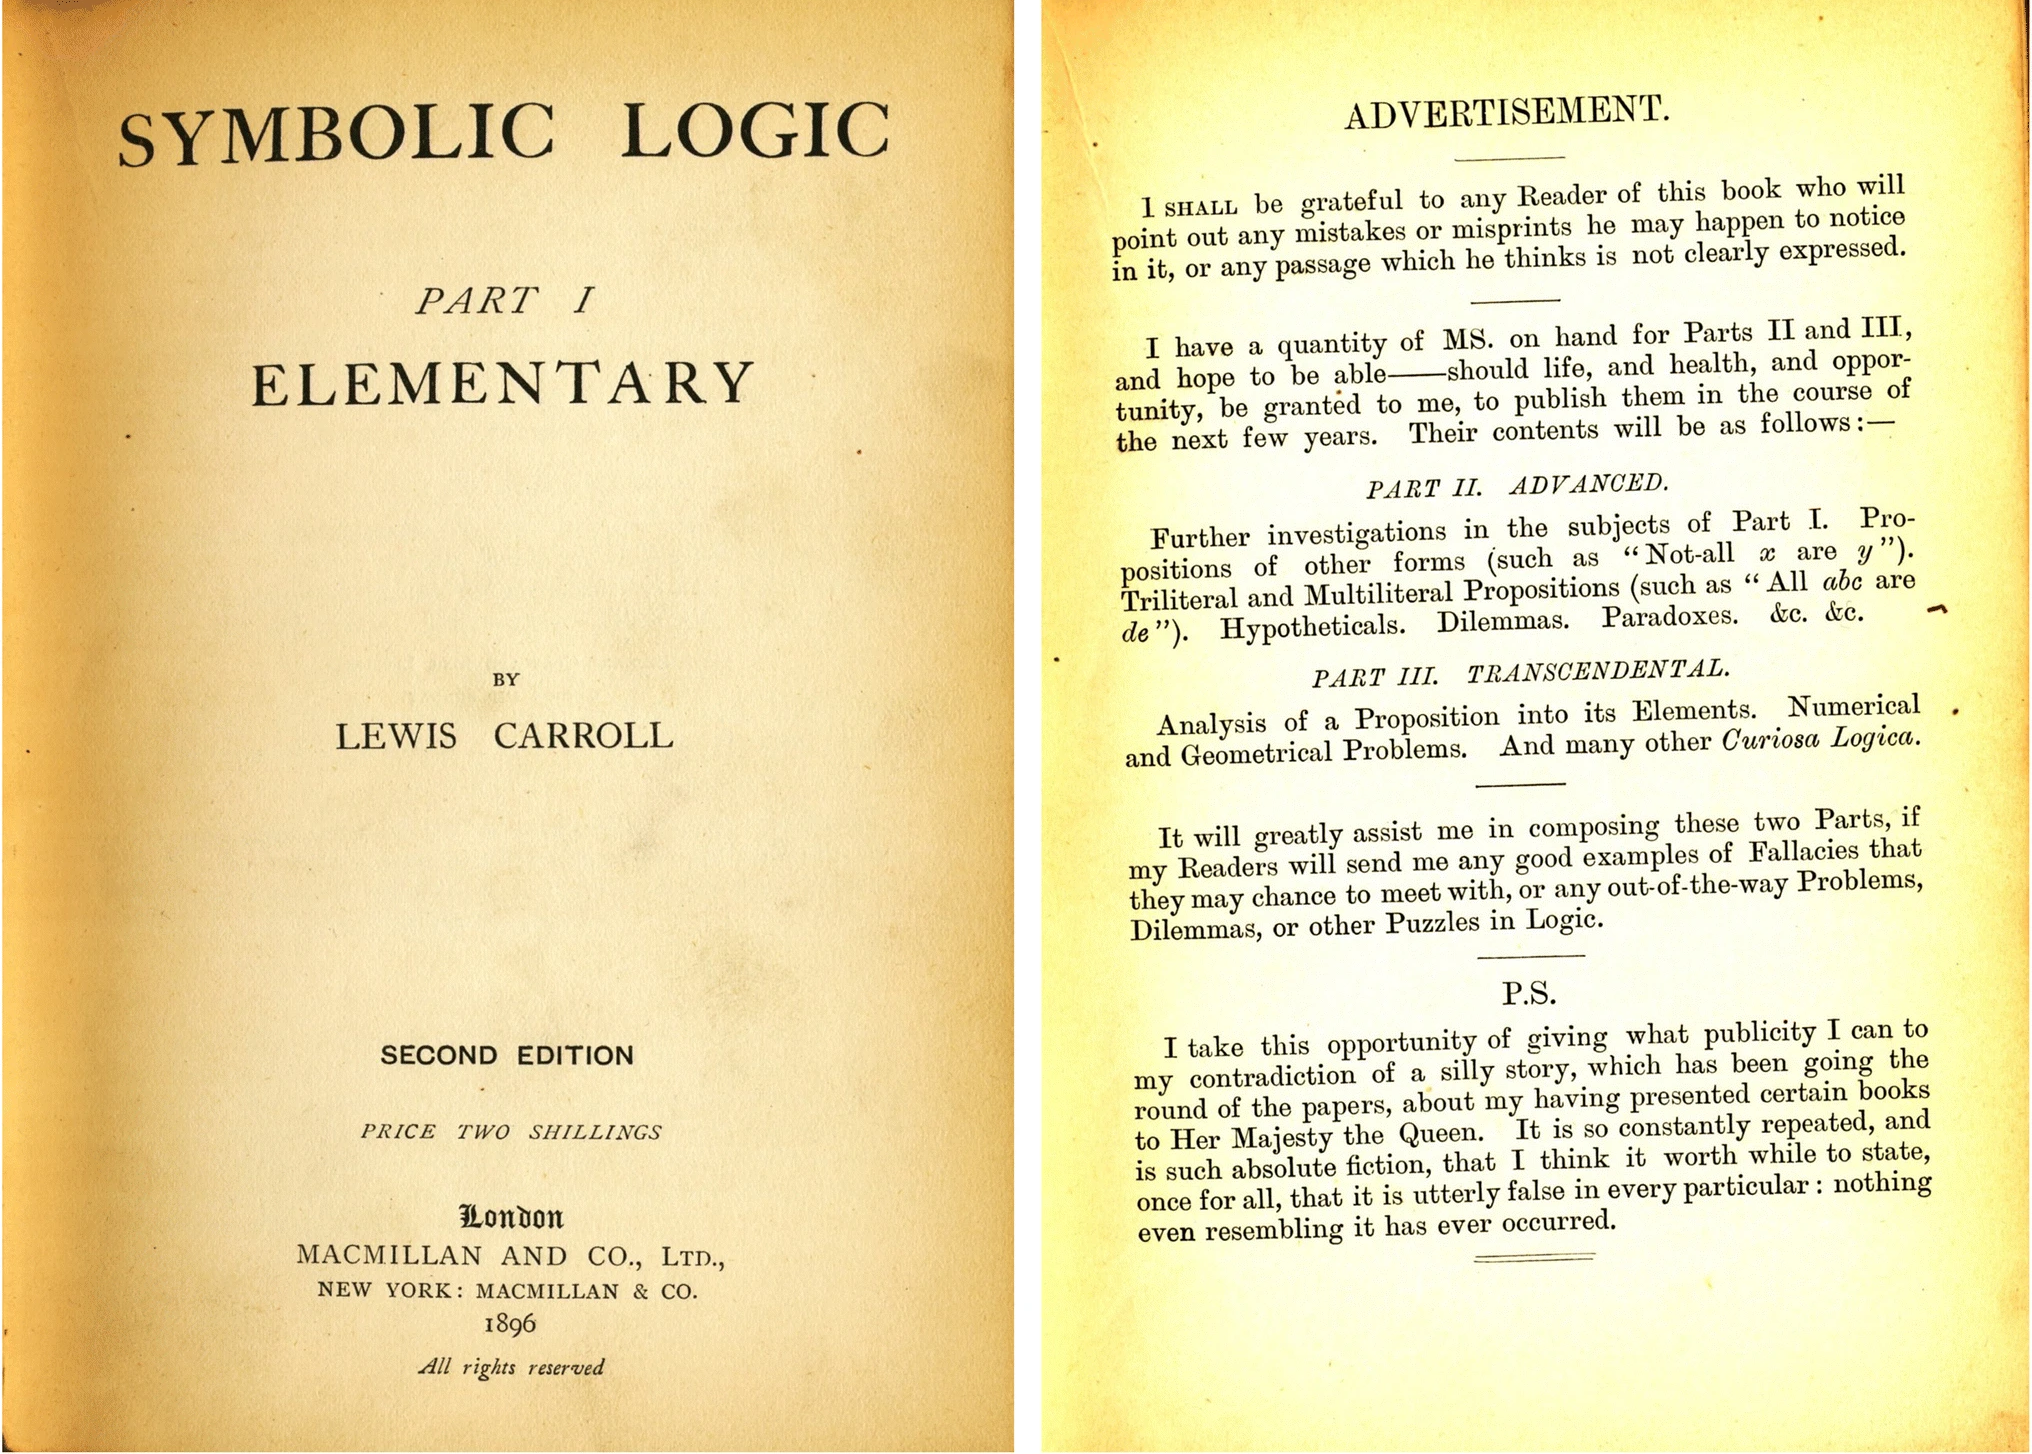
\includegraphics[width= 0.65\linewidth]{4}
		\caption{\small\textit{\color{lichsutoanhoc}Plato ($428-347$ TCN).}}
		\vspace*{-10pt}
	\end{figure}
	\textbf{\color{lichsutoanhoc}Menaechmus}
	\vskip 0.05cm
	Eudoxus được ghi nhớ trong lịch sử toán học không chỉ vì công việc của riêng mình mà còn thông qua học sinh của mình. 
	\vskip 0.05cm
	Ở Hy Lạp, có một sợi dây tiếp nối truyền thống từ thầy sang trò.  Thí dụ, Plato học được từ Archytas, Theodorus và Theaetetus; ảnh hưởng của Plato lần lượt được truyền qua Eudoxus cho anh em Menaechmus và Dinostratus, cả hai đều đạt được thành tựu xuất sắc trong toán học. 
	\vskip 0.05cm
	Menaechmus nổi tiếng là người đã khám phá ra các đường cong mà sau này được gọi là hình elip, parabol và hyperbol, các thiết diện được cắt ra bởi hình nón (các đường cong conic).
	\vskip 0.05cm
	Menaechmus đã thành công dựa trên các đường cong conic với các tính chất thích hợp để giải bài toán gấp đôi khối lập phương. 
	\vskip 0.05cm
	Proclus đã viết rằng Menaechmus là một trong những người đã ``làm cho toàn bộ hình học trở lên hoàn hảo hơn" (made the whole of geometry more perfect). Chúng ta biết rằng Menaechmus đã dạy Alexander Đại đế, và huyền thoại nổi tiếng thuộc về Menaechmus, khi học trò của ông yêu cầu một lối tắt đến hình học: ``Hỡi Vua, để đi qua đất nước, có những con đường hoàng gia và những con đường dành cho công dân chung; nhưng trong hình học, chỉ có một con đường cho tất cả mọi người".
	\begin{figure}[H]
		\vspace*{-5pt}
		\centering
		\captionsetup{labelformat= empty, justification=centering}
		\includegraphics[width= 0.65\linewidth]{3}
		\caption{\small\textit{\color{lichsutoanhoc}Menaechmus ($380-320$ TCN).}}
		\vspace*{-10pt}
	\end{figure}
	Chứng cứ Menaechmus phát hiện ra các thiết diện conic là do một lá thư từ Eratosthenes đến Vua Ptolemy Euergetes, được Eutocius trích dẫn khoảng $700$ năm sau đó, trong đó bài toán gấp đôi khối lập phương được đề cập. 
	\vskip 0.05cm
	\textbf{\color{lichsutoanhoc}Dinostratus và cầu phương hình tròn}
	\vskip 0.05cm
	Dinostratus, anh trai của Menaechmus, cũng là một nhà toán học; một người đã ``giải quyết" bài toán gấp đôi thể tích khối lập phương, người còn lại ``giải quyết" bài toán cầu phương hình tròn. 
	\vskip 0.05cm
	\textbf{\color{lichsutoanhoc}Thay lời kết}
	\vskip 0.05cm
	Tất nhiên, người Hy Lạp cũng hiểu rằng việc sử dụng đường cong trong các bài toán chia ba góc và các bài toán cầu phương đã vi phạm quy tắc của trò chơi -- chỉ cho phép sử dụng compa và thước thẳng. ``Lời giải" của Hippias, Menaechmus và Dinostratus, như các tác giả của chúng cũng nhận ra, là ngụy tạo; vì thế, việc tìm kiếm các giải pháp khác, chính tắc hoặc bất hợp pháp, tiếp tục, với kết quả là một số đường cong mới đã được phát hiện bởi các nhà hình học Hy Lạp.
	\vskip 0.05cm
	\textbf{\color{lichsutoanhoc}Tài liệu tham khảo chính}
	\vskip 0.05cm
	[$1$] David M. Burton, \textit{The History of Mathematics, An Introduction, Seventh Edition}, McGraw--Hill, $2011$. Chapter $3$: The Beginnings of Greek Mathematics, pp. $116-139$.
	\vskip 0.05cm
	[$2$] Thomas Heath, \textit{A History of Greek Mathematics, Oxford at the Clarendon Press}, $1921$, Volume $1$: From Thales to Euclid, pp. $170-353$.
	\vskip 0.05cm   
	[$3$] Victor J. Katz, \textit{A History of Mathematics, An Introduction}, Third Edition, Addison--Wesley, $2009$. Chapter $2$: \textit{The Beginnings of Mathematics in Greek}, pp. $40-49$.
	\vskip 0.05cm
	[$4$] Uta C. Merzbach and Carl B. Boyer, \textit{A
	History of Mathematics}, Third Edition, John Wiley \& Sons, $2011$, trang $57-89$.
	\vskip 0.05cm
	[$5$] Ngô Việt Trung, \textit{Lý thuyết Galois về các vấn đề giải phương trình bằng căn thức, dựng hình bằng thước kẻ và compa}, Nhà xuất bản Đại học Quốc gia Hà Nội, $2006$.
	\vskip 0.05cm
	\textbf{\color{lichsutoanhoc}Tài liệu tham khảo}
	\vskip 0.05cm 
	[$6$] George Johston Allman, \textit{Greek Geometry: From Thales to Euclid}, Dublin Universty Press, $1877$, $432$ trang.  
	\vskip 0.05cm
	[$7$] Euclid, \textit{Cơ sở của Hình học}, Nhà xuất bản Trí thức, $2016$, $350$ trang.
	\vskip 0.05cm
	[$8$] R. Lloyd, \textit{Early Greek Science: Thales to Aristotle}, $1970$, Chatto \& Windus, London, $156$ trang. 
	\vskip 0.05cm
	[$8$] Nicomachus of Gerasa, \textit{Introduction to Arithmetic}, Translated into English by Martin Luther D’ooge, The Macmillan Company, New York, $1926$.
	\vskip 0.05cm
	[$9$] Proclus, \textit{Commentaries on Euclid’s books}, Vol. $1$, $330$ trang.
	\vskip 0.05cm
	[$10$] Arpad Szabo, \textit{The beginnings of Greek Mathematics}, Springer, $1978$, $363$ trang.
	\vskip 0.05cm
	[$11$] M. L. West, \textit{Early Greek Philosophy and the Orient}, Oxford at the Clarendon Press, $1971$, $255$ trang.
\end{multicols}
